% Appendix A

\chapter{Additional evaluation results} % Main appendix title

\label{AppendixA} % For referencing this appendix elsewhere, use \ref{AppendixA}

\lhead{Appendix A. \emph{Additional evaluation results}} % This is for the header on each page - perhaps a shortened title

\section{Evaluation results for SNR = 10 dB}

\begin{figure}[htbp]
	\centering
		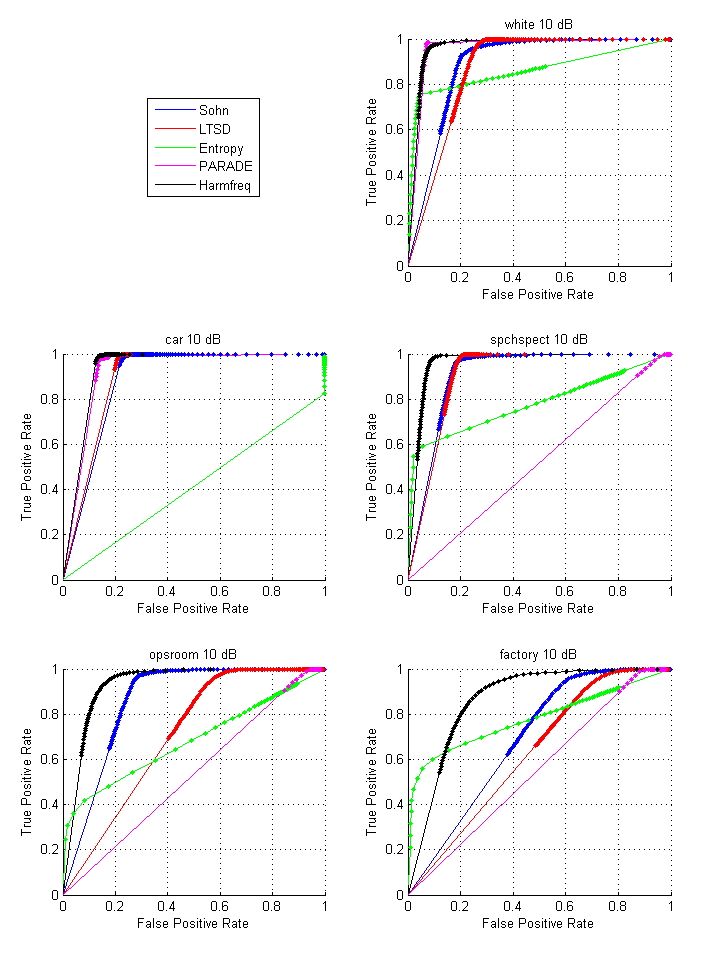
\includegraphics[width=1.0\columnwidth]{Figures/Chapter3/10dB.png}
		\rule{37em}{0.5pt}
	\caption[ROC curves of the evaluated VAD algorithms for SNR = 10 dB in various types of noise]{ROC curves of the evaluated VAD algorithms for SNR = 10 dB in various types of noise}
	\label{fig:10dB}
\end{figure}

\section{Evaluation results for SNR = 5 dB}

\begin{figure}[htbp]
	\centering
		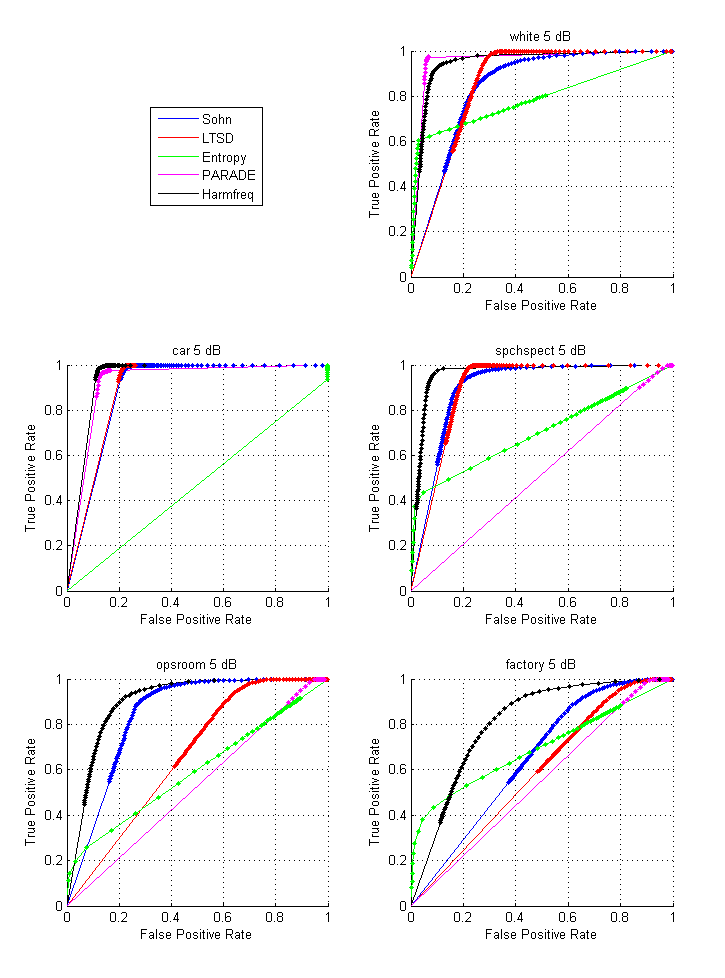
\includegraphics[width=1.0\columnwidth]{Figures/Chapter3/5dB.png}
		\rule{37em}{0.5pt}
	\caption[ROC curves of the evaluated VAD algorithms for SNR = 5 dB in various types of noise]{ROC curves of the evaluated VAD algorithms for SNR = 5 dB in various types of noise}
	\label{fig:5dB}
\end{figure}